\input{chapter-header.tex}
% =============================================================================
\chapter{Introduction}
\chaplabel{introduction}
\minitoc
% =============================================================================


Reflective systems are those that reason about and act upon themselves \cite{Smit84a}. A causal connection exists between the program and its representation inside the program itself as a meta-program \cite{Maes87a}. This reflective architecture introduces self-references:  an object-oriented system is composed by objects, which are instances of classes, which are also objects, and so on. These self-references, also known as meta-circularities \cite{Chib96a}, allow the manipulation of several meta-levels on one infrastructure.

Reflective systems traditionally modify their self-representation to evolve and define new abstractions. However, the self-modification approach of evolution has many drawbacks, such as making difficult the self-surgery operations~\cite{Casa09a} or the lose of the reproducibility of the system. On the other hand, non-reflective systems develop an evolution approach by recreation. Whenever a change has to be made to the system, a new system is created with the new changes applied. This approach solves many of the drawbacks of the reflective approach.

\gp{add some sentences on why it is important to evolve, which kind of software artifacts we would like to evolve, why it is challenging}

% =============================================================================
\section{The need for Software Evolution}
% =============================================================================

Software inevitable changes and we need to provide with the tools and methodologies that support such changes~\cite{Nier08b}. However, production-ready applications are not usually change-aware. These applications should be either engineered from scratch with change in mind, or a lot of reengineering effort should be invested in them to support change. Making deep modifications to a language runtime can be a cumbersome task.
In the last years, evolving a language runtime has become an important task. Multicore hardware brought new problems on concurrency and parallelism; the \emph{cloud} increased the need for software adaptation; new resource constrained devices presenting new challenges to software developers. The software we use, and in particular the programming languages and tools we use should be easily tailorable to support many of the new challenges that come with new technology and needs.

% =============================================================================
%\section{Resource Constrained Devices}
% =============================================================================

%\gp{noury had a reference on this -> everything is going small}

%Unused deployed code units have an undesired impact when targeting a constrained infrastructure. 
%Constrained devices may present restrictive hardware such as low primary or secondary memory, or even software impositions such as the Android's Dalvik VM restriction to deploy only 65536 methods\footnote{According to dalvik's bytecode documentation~(\url{http://source.android.com/devices/tech/dalvik/dalvik-bytecode.html}), the source register accepts values between 0 and 65536.}. Big JavaScript mashup applications have an impact on loading time due to network speed and parsing time.
%These limitations may forbid the deployment of applications that contain lots of code units, or limit the amount of applications and content an user can have in its device.

%Existing solutions to this problem propose the extraction of used code units of an application to reduce their size and memory footprint. Java Micro Edition~\cite{JavaME} proposes a general purpose specialized runtime environment with no possibility of customization. Other solutions in the field propose to automatically detect and extract used code units, so called \emph{tailoring}, with static call graph construction as the most dominant technique~\cite{ShortGrov97a}. 
%Static approaches present limitations in the presence of dynamic features such as reflection or in the absence of static type annotations. Additionally, these existing solutions are generally designed to extract all used code units with no possibility for the user to customize the process of selection.

For example, an application runtime should be easily tailorable to consume less resources. We can observe that deployed applications contain a set of \emph{code units} such as classes and methods that tend to occupy more memory~(primary and secondary) than necessary.
%Besides, an application may load a code unit that is only partially used, such as a class with some methods that are never invoked.
%Deployed object-oriented applications often contain \emph{code units}~(e.g. packages, classes, methods) that the running application never uses. 
This problem shows itself more evident and harder to control under the usage of third party software. 
Third party libraries and frameworks are designed in a generic fashion that allows multiple usages and functionalities, while applications use only few of them. 
Examples are logging libraries, web application frameworks or object-relational mappers.


%Figure~\ref{fig:unusedCodeUnits} shows a typical deployment scenario with unused code units.
%
%This problem becomes more evident with the inclusion of third party libraries~(and frameworks). 
%Third party libraries provide often a great variety of code units, usually designed in a generic fashion. 
%They allow multiple usages, while applications tend to use only some of them. 
%Additionally, application developers do not often modify and customize third party libraries to fit their needs but use them as black boxes. 
%Modifying them would mean to lose compatibility with the original development branch of the library and having deep knowledge on the library.
%
%\begin{figure}[ht]
%\begin{center}
%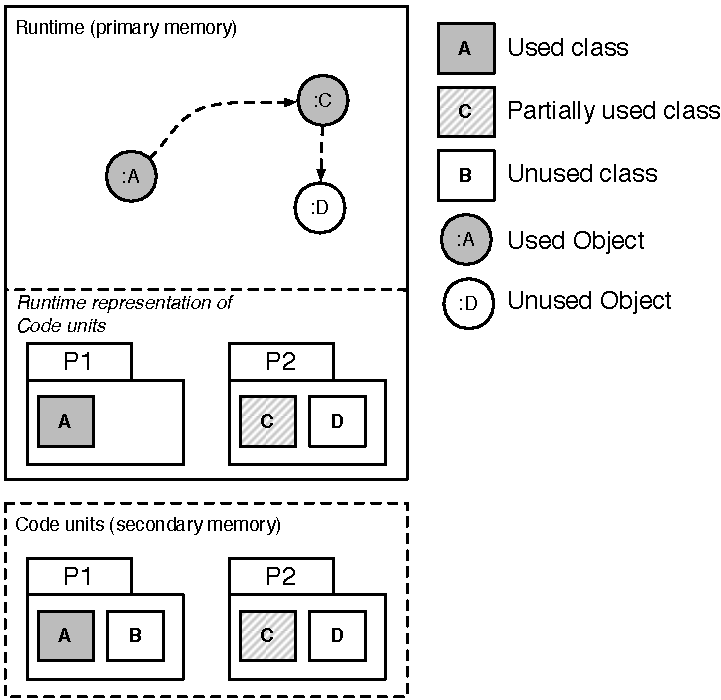
\includegraphics[width=1\linewidth]{components}
%\caption{\textbf{Unused Code Units.} Package P1 contains class A which is used during runtime and class B which is never needed and thus, not loaded. Package P2 contains class C which is partially used~(it contains methods that are never invoked) though it's completely loaded. Class D is loaded because an instance of it is created, but it is never used.\label{fig:unusedCodeUnits}}
%\end{center}
%\end{figure}

Unused code units represent serious drawbacks in constrained devices. 
First, unused code units may forbid the deployment into a constrained resource device.
It may also interfere with the deployment and usage of other applications, because of large memory footprints in both secondary~(disk storage) and primary~(RAM) memory~\cite{Mart12a} or the presence of slow networks in the case of rich web applications.
Second, some deployment targets may have an infrastructure designed in such a manner that forbids the deployment of large applications. For example, the Android's Dalvik VM restricts an application to deploy only 65536 methods.


% =============================================================================
%\section{The cloud and Mobile code}
% =============================================================================

%\gp{explain why code mobility is important!}

Another example of support that should be brought to user applications is \emph{code mobility}. Code mobility is a mechanism that allows the migration of programs between different environments. This problem is important in the context of ubiquitous systems and virtualization technology. Code mobility provides support for \eg load balancing, adjusting an application's resources dynamically and functionality customization. Fuggetta et al. define informally code mobility as the capability to rebind a piece of code with the location it is running~\cite{Fugg98a}. Such rebinding may consist, depending on the style of mobility, in the mobility of execution state, application data and resources, or both of them. Execution state mobility is the ability to suspend the actual execution of a program and transfer its internal execution information~(\eg code, execution stacks, instruction pointers) to some other environment. Data mobility is the ability to transfer the application's data~(\eg objects, database connections, files) between different environments.


% =============================================================================
\section{What to Evolve?}
% =============================================================================

High-level language runtimes are inherent complex pieces of software.
First, \VMs have to combine two rather extreme goals: abstraction and performance.
We have seen that the required abstraction for the running high-level language has a strong influence on the \VM design.
At the same time the hard performance requirement requires precise interaction with the underlying hardware.
This goes even so far that specialized hardware is conceived to match the performance requirements \cite{Unga84a,Stef84a,McGh98a,Clic05a}.


We run our languages and applications on top of these complex \VMs.
Then, our programs must comply to the contract required by the \VM to run, namely the \VM's \emph{execution model}.
A \VM's execution model imposes for example an object format, a class or prototype model to perform a method lookup, a bytecode set to execute methods at runtime.
In some cases, the \VM also loads and initializes the language structures.
These \VM-language complex interactions makes difficult to evolve any of these elements without affecting the other.

In the following sections we propose a dissection of a high-level program. We made this dissection with the objective of understanding the relation and separation between the elements we believe important in the context of software and language evolution. The identified elements will also serve for the understanding of the rest of this dissertation.

\gp{guile stopped here}


\subsection{Virtual Machines}

The early \VMs focused on interpreting an abstract instruction set (bytecodes).
The benefits are twofold.
On the one hand the bytecodes guarantee certain platform independence by abstracting away from the \CPU specific instruction set.
On the other hand bytecodes allow to encode complex operations into little space both serving the hard memory constraints of the hardware and simplifying the design of a compiler.
Obviously this abstraction gain comes at a cost and ever since the first \VMs were built research and industry strive to reduce the interpretation overhead.
An efficient way to improve performance is to use a just in time compiler (\JIT) that dynamically generates native code from the bytecode \cite{Deut84a}.
In this case the bytecode becomes an intermediate representation (\IR) for a bigger compiler infrastructure.
However, \JIT compilers are notoriously complex as they crosscut many \VM components.
At the same time they crosscut all abstraction layers; they have to access high-level information from the running bytecodes and manage native code at the same time.
Similar complexity applies to the automatic memory management present in most high-level language \VMs.
Garbage Collectors (\GC) evolved from simple helpers to complex software artifacts that for instance support concurrent garbage collection \cite{Clic05a}.

\subsection{Language Runtime and Kernel}

Launching the VM initializes its internal structures~(\ie allocates the heap, initializes threads and input/output streams, loads external libraries, etc.) and \textbf{the language kernel}. The language kernel is the set of objects and functions/methods\footnote{these constructions vary from language to language.} available to a program from the very beginning. It includes basic objects such as booleans, numbers and strings as well as basic language libraries\gp{give a better example}.

\subsection{Application Software}

% =============================================================================
\section{On Evolution Methodologies}
% =============================================================================

\subsection{Recreation: The case of non-reflective languages}

Non-reflective software evolve by recreation. This means they evolve by generating from scratch of a new version of it. These systems are generated by a system \emph{builder} which takes a \emph{specification} of the system and builds the new system (\autoref{fig:generate_system}).
The specification of the system must include the elements and behavior of the new system. Sometimes it can also include some order in which the system should be built.
For example, to recreate a C program, a C compiler (the system builder) will take the source code of the program (the specification) as input.

\begin{figure}[!ht]
\begin{center}
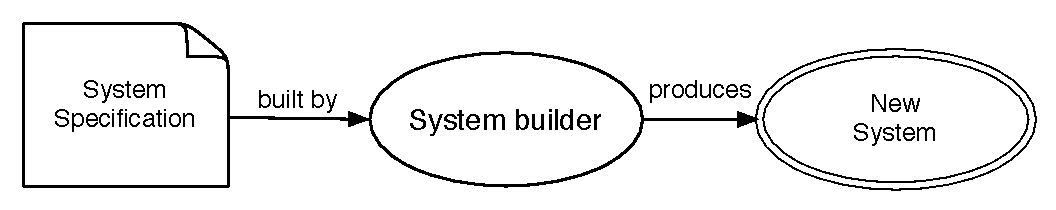
\includegraphics[width=0.6\linewidth]{system_recreation}
\caption{Process to generate a new system.\label{fig:generate_system}}
\end{center}
\end{figure}

\autoref{fig:evolution_recreation_systems} depicts how a system such as a C compiler can evolve using this approach.
At the first stage, the compiler and its source code represent version 1 of the system.
A change is introduced in the source code of the compiler, to depict version 2 of the source code.
The version 1 of the compiler, which conforms to the version 1 of the source code, is now \emph{out of synchronization} with the new source code or specification.
The source code version 2 is used to generate the compiler version 2.
Finally, the compiler version 2 conforms to the source code in version 2.

%\begin{figure}[!ht]
%\begin{center}
%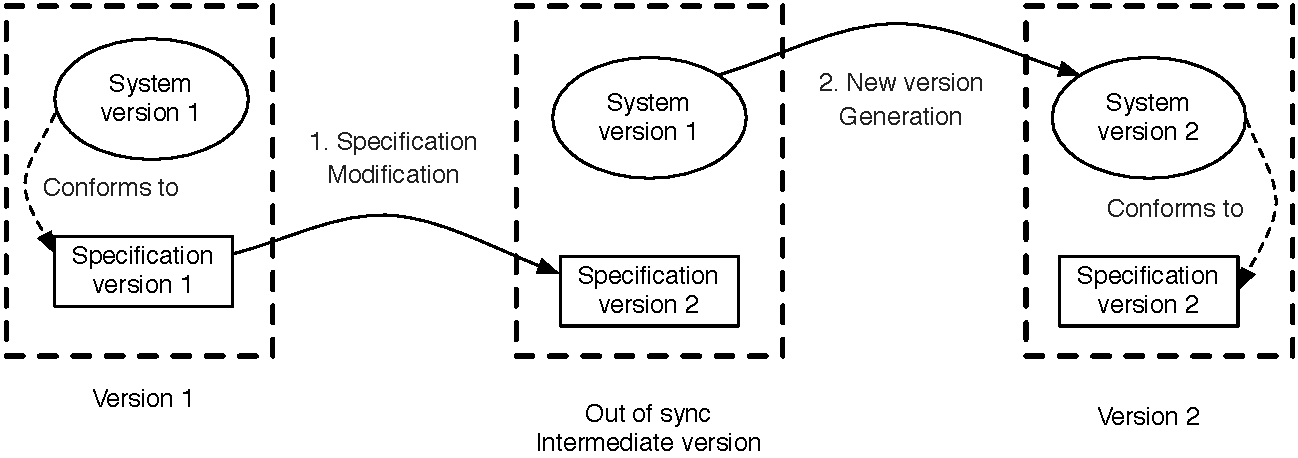
\includegraphics[width=0.5\linewidth]{evolution_recreation_systems2}
%\caption{Evolution of a non causally connected system by recreation after each modification of the system specification\label{fig:evolution_recreation_systems}}
%\end{center}
%\end{figure}

This approach provides a deterministic and explicit process to build a new version of the system from scratch.
Multiple changes can be applied to the specification while it is out of synchronization with the system.
These changes will be applied atomically in the new system when it is generated.
On the other hand, the main drawback of this approach is the slow feedback loop in the development process.
The specification and the system can stay out of synchronization during a large period of time without providing information about errors and mistakes.
Thus, it is easier to reach non-working stages.

%A particular case of system recreation is the introduction of the newly generated system into the generation process. The newly generated system can be used as a system builder in the process of generating a new system. This case, commonly known by its usage in compilers, is normally referred as \emph{bootstrapping}.


\subsection{Self-Modification: The case of reflective languages}

\gp{emphasize this is the way for 0-down systems, since we cannot stop them to update/change them}

Reflective systems are those that reason about and act upon themselves~\cite{Smit84a}.
They embed their structure and behavior in themselves in a causally connected way.
Causal connections enable a reflective system to modify itself and reflect their changes immediately.
The ability to change itself is called \emph{self-modification}.

A system evolves by self-modification when it applies \emph{deltas} directly on itself to alter its representation. 
A delta is an atomic and indivisible change of the system, such as the introduction of a class or a method, or the assignment of a variable.
Each delta applied to the system triggers a migration of the entities in the system, which automatically reflect the change.
For example, adding an instance variable into a class definition migrates all its instances by adding them the new extra slot.
Thus, the system is at any moment during its life synchronized with its internal representation.\gp{say it is a causal connection}
To evolve a system to a desired state, a \emph{stream} of deltas in a specific order must be applied to it.
\autoref{fig:evolution_reflective_systems} shows how a stream of changes \{$\Delta_1, \Delta_2$\} is applied to version 1 of a reflective system to obtain, in order, version 2 and version 3.

\begin{figure}[!ht]
\begin{center}
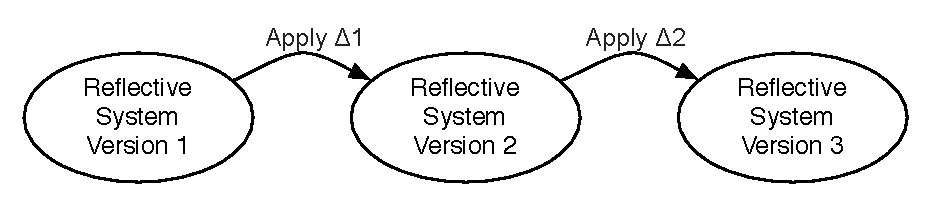
\includegraphics[width=0.6\linewidth]{evolution_reflective_systems}
\caption{Evolution of a reflective system by self-modification\label{fig:evolution_reflective_systems}}
\end{center}
\end{figure}

%Pharo~\cite{Blac09a} and Squeak~\cite{Blac07a} are object-oriented systems evolving traditionally by self-modification. These systems store their state and all their objects in an \emph{image}. A snapshot of the image can be stored at any time, creating a \emph{backup} of the state of the system. When the image is restarted, its state is the same as it was at the last snapshot. These systems evolve by applying deltas on themselves and making a snapshot of the new state of the system.

%Some tools such as the SystemTracer in Squeak~\cite{Blac07a} can produce a new image by applying certain transformations (like pointer representation modification) to the objects.

\gp{review from here}
Based on our experience maintaining and evolving them during several years \cite{Denk07a}, we list some problems appearing in these evolutive approach: 
\begin{description}

\item[\emph{Evolving requires sequences of side effects.}] A stream of ordered and compatible delta have to be applied to the system to reach a particular version of it. A delta could depend on the deltas applied before it, and enable the application of its subsequent ones. It may be difficult to order the deltas of big changes to get the system to a specific state. 
Consider for example a Smalltalk system with an \ct{Array} class defining an iterator method \ct{do:}.
This iterator method is used in critical parts of the system.
A refactor to move the iteration method to the superclass of the Array class consists basically in the removal of the method from the \ct{Array} class and the introduction into its superclass.
However, removing first the method from the \ct{Array} class leads to an irrecoverable system crash.
To perform this refactor safely, the order in which the actions are realized must be reverted: first the iterator method must be introduced into the superclass.
So, when removing the method in the Array class, the method is looked up correctly.
Evolution by self-modification lacks a way to apply several changes atomically to a system.

\item[\em{Impossibility to recover from system crashes.}] When doing self brain surgery~\cite{Casa09a} in the system (modifying parts of the system that are used to performing the changes themselves), a delta in a given stream may leave the system in a broken state. This leads to the lose of the already applied deltas. The system relies on its backups or snapshots to recover to a previous state, making difficult and tedious the process to evolve the system to versions involving many critical deltas. 

\item[\emph{Unmaintained code.}] The initialization methods of certain classes are not systematically exercised. This makes the code of these initializations get easily broken or obsolete. For example, the character table in the system can be modified by altering it directly without updating its initialization code. Additionally, methods can refer to inexistent classes or send messages that are not understood any more. Such a situation presents a problem when these parts of the system have to be re-initialized again.

\item[\emph{Lack of support for building up the system.}] The system is represented by a monolithic image containing lots of packages not needed for every usage, such as the UI, networking, debugger or compiler. This monolithic image, due to its size, represents a problem when deploying it on a resource constrained environment such as embedded devices. Building a system with only the necessary parts is nowadays only feasible by image shrinking with self-modification, making the system unstable during its modification.
The image has been a big monolithic unit since years, leading to hidden and hard to break dependencies in it, making the shrinking process tedious. Additionally, the dynamic nature of the system and the use of reflective features breaks static analysis when trying to understand the hidden dependencies \cite{Livs05a}.
\end{description}


% =============================================================================
%\section{Problem Statement}
% =============================================================================

\section{Problems Modifying a Language Runtime} \label{sec:bootstrapping_problems}

We identify three main limitations in the state of the art of language initialization techniques. First, how flexible is a language definition to be changed and adapted. Second, the unclear mixture of \VM and language concerns prevents us to extract the language definition and easily replace it. Finally, the differences in the abstraction levels and tool support between the language we are building and the language we use to build it makes it a challenging task.

%A high-level object-oriented language kernel is the runtime representation of the abstractions that define the language behaviour. For example, Ruby language kernel is composed by the initial class hierarchy~(\ct{BasicObject}, \ct{Object}, \ct{Module} and \ct{Class}), their respective metaclasses and methods. Changing this language kernel is a challenging task.

\subsection{Flexibility to Change a Language Runtime}

The \VM is often the component in charge of initialising the language kernel. This decision is indeed practical as the \VM can safely initialise the language structures and solve the language bootstrapping issues avoiding recursions~\cite{Kicz91a}~(\eg create the first class without a class). This language kernel must comply at runtime to the execution model imposed by the \VM~(\eg an object format denoting how objects are represented in memory and a set of instructions for execution such as bytecode or assembly). This coupling is indeed necessary to run a program but does often remain hidden in hardcoded assumptions.

These hardcoded \VM assumptions have two main consequences when we target to change the language kernel: the \VM fixes its initial structures~(\eg Ruby's class hierarchy in Figure \ref{code:ruby_hierarchy}) and they introduce code duplications to manipulate language objects.
To illustrate this second problem, let us consider the code in Figure~\ref{code:logic_dup} that creates a \ct{Dictionary} or hashmap. A language kernel that is defined by a \ct{Dictionary} object to keep \eg a map of global objects, must execute the code in the figure to create the corresponding instance. However, since the language kernel and the \VM are in middle of their initialization, the \VM cannot execute this code as it is, and thus it cannot enforce its own invariants. The state of the art \VMs will provide an alternative low-level representation of the same code respecting the same invariants~(Figure~\ref{code:logic_dup2}). This introduces a redundancy: the \VM and the language have different code to honor the same invariants.

\begin{figure}[ht]
\begin{code}
Dictionary class>>new: n
    ^ self new initialize: n

Dictionary>>initialize: n
    "Initialize array to an array size of n"
    array := Array new: n.
    tally := 0
\end{code}
\caption{\textbf{Code to create a \ct{Dictionary} object in Smalltalk.}\label{code:logic_dup}}
\end{figure}

\begin{figure}[ht]
\begin{code}
void* createDictionaryWithSize(int n){
    void* dictionary, internalArray;
    dictionary = instantiateClass("Dictionary");
    internalArray := instantiateClass("Array", n);
    setInstanceVariable(dictionary, 1, internalArray);
    setInstanceVariableInt(dictionary, 2, 0);
    return dictionary;
}
\end{code}
\caption{\textbf{Code to create the same \ct{Dictionary} object from C.}\label{code:logic_dup2}}
\end{figure}


%This execution model is often less restrictive than the object models of the language's that run on top of them. For example, the Smalltalk and Ruby \VMs require for each object in the system to have a class, and each class a superclass, but there is no need for metaclasses.

After the language initialization, reflective languages~\cite{Smit84a} such as LISP or Smalltalk provide the means to modify themselves at runtime. These languages are based on a reflective architecture presenting the notion of causal connection~\cite{Maes87a}: a link between a programming element and its representation that keeps both in synchronization. However, as these languages contain meta-circular definitions in their kernel~\cite{Chib96a}, this can result in a Metastability problem~\cite{Kicz91a} \ie a change in the language kernel may introduce a meta-call recursion and turn the system unusable. In this context, Reflectivity~\cite{Denk08b} is a framework that scopes reflection to avoid meta-call recursions.  Reflectivity succeeds to control behavioural reflection by accounting the level of \emph{metaness} of the execution in a program and executing reflective operations when it is in the correct meta-level. The main limitation of Reflectivity is that it does not allow structural reflective changes in the language kernel.

Finally, snapshot-based languages offer different means to evolve a language kernel. Instead of being reinitialized each time we need it, the state of the whole graph of objects that denotes the running program can be suspended and saved as a snapshot in a file. Later on, the program in this snapshot can be restarted from the point it was suspended. As a consequence of this persistency property, some snapshot-based languages such as Squeak or Pharo  do not have the infrastructure to be reinitialised from scratch. Indeed, their current deliverable snapshots are the result of a chain of side effects (updates and migrations) made to the original Smalltalk-80 snapshot. Thus, even if we can change the language kernel at runtime, they cannot ensure a reproducible initial state for their users.

\subsection{Mixture of \VM and Language Concerns}

The unclear interface between the language and the \VM makes difficult to recognize whether a piece of code belongs to a \VM or language concern. This causes undesirable temporal couplings between these two elements and prevents us to clearly extract and replace the language definition by another one.
To illustrate this problem, Figure \ref{code:jikes_vm_initialization} shows an excerpt of the JikesRVM\footnote{Taken from the version 3.1.3 of the JikesRVM in \url{http://sourceforge.net/projects/jikesrvm}}~\cite{Alpe00a}. In this example, the memory manager is initialised in the middle of the initial class loading phase. These memory manager calls are indeed needed to avoid the collection of objects during the initialization. However, it is necessary to call it after some specific classes are initialized and not before.

\begin{figure}[ht]
\begin{code}
private static void finishBooting() {
    ...
    MemoryManager.postBoot(); //Memory management
    ...
    runClassInitializer("java.lang.Runtime");
    runClassInitializer("java.lang.System");
    runClassInitializer("sun.misc.Unsafe");
    ...
    MemoryManager.fullyBootedVM(); //Memory management
    ...
    runClassInitializer("java.util.logging.Level");
    runClassInitializer("gnu.java.nio.charset.EncodingHelper");
}
\end{code}
\caption{\textbf{Code of the JikesRVM that initialises loads the initial classes of the runtime (excerpt).} The code performing the initial class loading is mixed with the code that initialises the memory manager of the \VM.\label{code:jikes_vm_initialization}}
\end{figure}

Snapshot-based languages, on the other side, show that language initialization and \VM initialization can be orthogonal. Indeed, languages such as Pharo, LISP or the V8 flavor of Javascript can restart their system from a snapshot. The \VM loads atomically the snapshot and binds it to the current runtime. Loading a snapshot clarifies the \VM startup steps as it replaces the phase of language initialization. Moreover, as long as the snapshot satisfies the \VM execution model, it can run any language model, as it is the case of Pharo and Newspeak that run on the same \VM.

%Other snapshot-based languages such as GNU-Smalltalk or the V8 flavor of Javascript possess both mechanisms: they recreate the language runtime from scratch, and can also restart from a snapshot. In the case of V8, the snapshot was chosen with performance in mind, to avoid parsing and recreation on client-side machines.

%\item[The \VM-Language interface is unclear.]
%For example, the \VM assumes how objects are structured in the runtime to manipulate them: the amount and size of their instance variables, object headers, special kind of object references~(\eg weak references). The \VM also needs access to some well-known objects to run code: this is the case for example of \ct{nil}, \ct{true} and \ct{false} objects. Another example of a tight coupling are the callbacks \VM-language, where the \VM can trigger some specific code on the language to notify it from some event.

\subsection{Abstraction Level and Tool Support}

On one side, when defining the language kernel at the \VM level, we rely on the tools and abstractions available to develop the \VM to change the language. That means that the language developer uses low-level abstractions to express possibly higher-level concerns. Indeed the developer would benefit from the productivity that a high-level language brings.

To attack these problems, many programming systems have found desirable to follow the principles of \emph{high-level low-level programming} \ie expressing low-level concerns using high-level languages~\cite{Fram09a}. High-level low-level programming pursues the objective of simplifying the complexity of programming systems. By using a high-level language to describe the low-level world the developer benefits from their abstraction power and tooling of the first one. A clear example of this fact is the metacircular \VM field, where many projects whose goal is to write \VMs in a high-level language have blossomed in the last years~\cite{Wimm13a,Alpe00a,Verw11a,Inga97a,Unga05a,Rigo06a}. These projects are biased to \VM building techniques and not to the initialization of the languages that run on top of them.

On the other side, we found that reflective languages support naturally the usage of the language abstractions and tools to modify the language kernel. Reflective languages benefit from the reification of the language concepts to be able to change them from the language itself.


\subsection{Problem Statement}

\gp{write from scratch}
Following the problem description listed in the above introduction we identified the following abstract concerns with existing reflective languages and their \VMs.
%
\begin{itemize}
	\item Reflection and in special behavioral reflection comes at a significant cost due to reification overhead.
		
	\item Intercession is limited to language-side.
	\VMs are not accessible from language-side and they are usually have no reflective properties at runtime. 
	
	\item Existing approaches to a unified model between the \VM and the language-side are holistic, there is no intermediate solution available.
\end{itemize}

\noindent Out of these general problems concerning reflection in high-level languages we see that they have a low-level root.
To address the unification of the language-side and \VM-side we have to grant more access to the language-side.
This includes interacting directly with low-level native instructions.
A similar problem has been solved by applying high-level low-level programming in a more static environment \cite{Fram09a,Graal}.
The approach outlined by Frampton et al. uses a high-level framework to generate native code at compile-time.
We see that their approach has not yet been applied in a more dynamic environment where native code has to be generated at runtime.
Hence we focus on the following concrete problems we wish to solve in this thesis.

\begin{description}
	\item[Problem 1:] High-level low-level programming is not available at runtime and from language-side.
	
	\item[Problem 2:] Intercession is limited to language-side.
	\VMs are not accessible from language-side and they are usually have no reflective properties at runtime.
	
	\item[Problem 3:] High-level low-level programming has not yet been provided as an incremental extension to an existing language runtime.
\end{description}

\gp{Guille}


A better language kernel initialization solution should have the following properties:
\begin{itemize}
\item Allow one to easily change the structure and behavior of the language kernel.
\item Clarify the separation between \VM and language.
\item Ensure the initial state of the language even in presence of a reflective architecture (Solving the bootstrapping and metastability problems as defined in AMOP~\cite{Kicz91a}).
\end{itemize}

% =============================================================================
\section{Thesis Outline}
% =============================================================================
%\sm{This dissertation structure is different to what I am used to. At least the way you announce the purpose of the chapters is not what I would expect.
%In my diss, everything revolves around one thesis, here, it is a number of things listed one after another, don't see the central motive I would expect}

\gp{write from scratch, left for the end}
\begin{description}
\item[\chapref{background}] sheds light on the context of this work.
	We present a quick overview of language-side reflection followed by a development of \VM-level reflection.
	We find that mostly metacircular \VMs provide limited \VM-level reflection and thus we present several high-level language \VMs falling into this category.
	We conclude that there is only two research \VM that has a uniform model for \VM and language-side.
	Among them is \P a research \ST \VM we contributed to previous to working on this dissertation.

%\item[\chapref{reification}] focuses on language-side applications that simplify the interaction with the underlying \VM.
%	We present a custom inspector framework that is now used by default in \PH.
%	As a second part we explain how we introduced first-class layouts and slots to \PH to reify the low-level structural layout of objects.
%	Both projects are crucial for metacircular \VM development and are direct results from the research conducted on the \P \VM.

\item[\chapref{benzo}] describes a high-level low-level programming framework named \B.
	The core functionality of \B is to dynamically execute native-code generated at language-side.
	\B allows us to hoist typical \VM plugins to the language-side.
	Furthermore we show how code caching makes \B efficient and users essentially only pay a one-time overhead for generating the native code.
	
\item[\chapref{ffi}] presents \NB, a stable foreign function interface (\FFI) implementation that is entirely written at language-side using \B.
	\NB is a real-world validation of \B as it combines both language-side flexibility with \VM-level performance.
	We show in detail how \NB outperforms other existing \FFI solutions on \PH.

\item[\chapref{validation}] focuses on two further \B applications.
	In the first part we present \WF a framework for dynamically generating primitives at runtime.
	\WF extends the concept of metacircularity to the running language by reusing the same sources for dynamic primitives that were previously used to generate the static \VM artifact.
	In a first validation we show how \WF outperforms other reflective language-side solutions to instrument primitives.
	
	In a second part of \chapref{validation} we present \NBJ a prototype \JIT compiler that is based on \B.
	\NBJ shows the limitations of the \B approach as it required a customized \VM to communicate with the existing \JIT interface for native code.
	Our prototype implementation generates the same native code as the existing \VM-level \JIT, however, it is currently limited to simple expressions.
	\NBJ shows that for certain applications a well-define interface with the low-level components of the \VM is required.

\item[\chapref{future}] summarizes the limitations of \B and its application.
Furthermore we list undergoing efforts on the \B infrastructure and future work.

\item[\chapref{conclusion}] concludes the dissertation.

\end{description}

% =============================================================================
\input{chapter-footer.tex}
% =============================================================================